\documentclass[aps,pre,twocolumn,showpacs,preprintnumbers]{revtex4-2}

% Packages
\usepackage{amsmath}
\usepackage{amssymb}
\usepackage{amsthm}
\usepackage{amsfonts}
\usepackage{graphicx}
\usepackage{dcolumn}
\usepackage{bm}
\usepackage{hyperref}
\usepackage{booktabs}
\usepackage{xcolor}

% Mathematical Commands
\newcommand*{\prob}{\mathbb{P}}
\newcommand*{\E}{\mathbb{E}}
\newcommand*{\Z}{\mathbb{Z}}
\newcommand*{\Q}{\mathbb{Q}}
\newcommand*{\R}{\mathbb{R}}
\newcommand*{\C}{\mathbb{C}}
\newcommand*{\N}{\mathbb{N}}
\newcommand{\Var}{\mathrm{Var}}
\newcommand{\Cov}{\mathrm{Cov}}
\newcommand{\pderiv}[2]{\frac{\partial #1}{\partial #2}}

\begin{document}

\title{Network Mini-project}

\author{Ray Tsai}

\begin{abstract}
We study the structural properties of the all-or-none network growth model, a variation of preferential attachment and copying mechanisms in which a new node connects to a uniformly chosen target and, with probability $p$, to \emph{all} of its neighbours, or with probability $1-p$ to \emph{none}. We derive analytical expressions for the expected number of edges as a function of $p$ and the number of nodes $N$, characterise the degree distribution in the sparse regime, and compute the clustering coefficient, assortativity coefficient, and average shortest-path distance. Our analytical predictions are supported by extensive numerical simulations.
\end{abstract}

\maketitle

% ============================================================
\section{\label{sec:intro}Introduction}
% ============================================================

Network growth models are central to our understanding of real-world complex systems, ranging from the World Wide Web to biological and social networks~\cite{barabasi1999,newman2003}. The Barab\'asi--Albert (BA) model~\cite{barabasi1999} introduced preferential attachment as a mechanism for generating power-law degree distributions, while copying models~\cite{kleinberg1999} propose an alternative microscopic rule in which new nodes replicate the connections of existing ones.

In this work we analyze the \emph{all-or-none} model: at each growth step a new node is added and connected to a target chosen uniformly at random; it then connects to \emph{all} neighbours of the target with probability $p$, or to \emph{none} of them with probability $1-p$. This binary choice creates a sharp interpolation between two qualitatively distinct regimes and leads to non-trivial structural properties that we characterise below.

The remainder of this paper is organised as follows. Section~\ref{sec:model} defines the model precisely. Sections~\ref{sec:edges}--\ref{sec:distance} derive analytical results and present numerical evidence for the edge count, degree distribution, clustering, assortativity, and average shortest-path distance, respectively. Section~\ref{sec:conclusion} concludes.

% ============================================================
\section{\label{sec:model}Model Definition}
% ============================================================

The network begins with a single node ($N=1$). At each growth step ($N\to N+1$):
\begin{enumerate}
  \item A new node $v$ is introduced.
  \item A target node $u$ is chosen uniformly at random from the existing $N$ nodes.
  \item An edge $(v, u)$ is added.
  \item With probability $p$, edges $(v, w)$ are added for every neighbour $w$ of $u$; with probability $1-p$, no further edges are added.
\end{enumerate}

% ============================================================
\section{\label{sec:edges}Number of Edges}
% ============================================================

Let $M_N$ denote the number of edges in the all-or-none network of $N$ nodes. At step $N\to N+1$, a target $u$ is chosen uniformly from the $N$ existing nodes. The expected number of new edges is $1 + p\,k_u$, where $k_u$ is the degree of $u$. Note that by the handshake lemma, the average value of $k_u$ over all choices of $u$ is $2M_N/N$. It follows that,
\begin{align}\label{eq:edge_rec}
  \E[M_{N+1}] 
  &= \E[M_N] + \left(\frac{2p}{N}\E[M_N] + 1\right) \notag \\
  &= \left(1 + \frac{2p}{N}\right)\E[M_N] + 1.
\end{align}
This is a first-order linear recurrence. A particular solution of the form $\alpha N$ yields $\alpha = 1/(1-2p)$ for $p\neq 1/2$. The homogeneous solution is $A_N = \Gamma(N+2p)/[\Gamma(1+2p)\,\Gamma(N)]$, satisfying $A_{N+1}/A_N = (N+2p)/N$. Imposing $\E[M_1]=0$ now yields
\begin{equation}\label{eq:edge_exact}
  \boxed{\E[M] = \frac{1}{1-2p}\!\left(N - \frac{\Gamma(N+2p)}{\Gamma(1+2p)\,\Gamma(N)}\right)}, \quad p\neq\tfrac{1}{2}.
\end{equation}
Since $\Gamma(N+2p)/\Gamma(N)\sim N^{2p}$ for large $N$, two regimes emerge:
\begin{itemize}
  \item \emph{Sparse} ($p<1/2$): $\E[M]\sim N/(1-2p)$ (linear).
  \item \emph{Dense} ($p>1/2$): $\E[M]\sim N^{2p}/[(2p-1)\,\Gamma(1+2p)]$ (superlinear).
\end{itemize}

\subsection{Numerical results}

\begin{figure}[h]
  \centering
  % 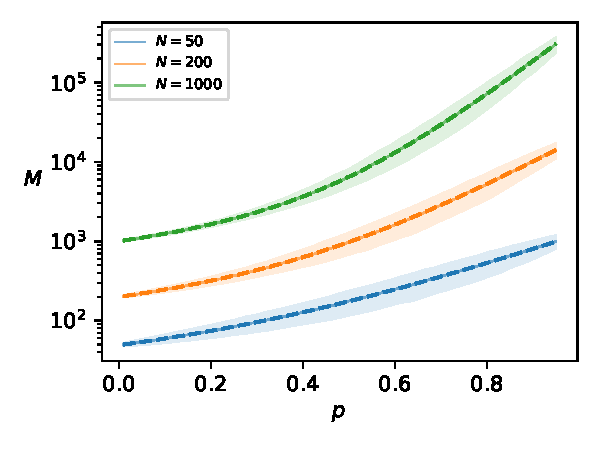
\includegraphics[width=\columnwidth]{figures/edges_vs_p.pdf}
  \caption{Expected number of edges $\E[M]$ as a function of $p$ for several values of $N$, obtained by averaging over $10^4$ independent realisations. Solid lines show the analytical prediction~\eqref{eq:edge_exact}.}
  \label{fig:edges}
\end{figure}

% ============================================================
\section{\label{sec:degree}Degree Distribution}
% ============================================================

Denote by $f(k, i, N)$ the probability that node $i$ has degree $k$ when the network has $N$ nodes. At step $N\to N+1$, degree $k$ increases by one with probability $(1+pk)/N$, because either the node is chosen as target (probability $1/N$) or a neighbour of it is chosen and the ``all'' event occurs (probability $pk/N$) The master equation for $f$ is then
\begin{align}\label{eq:master_node}
  f(k, i, N+1) 
  &= \frac{1+\!p(k-1)}{N}\,f(k-1, i, N) \notag \\
  &\qquad+ \left(1-\frac{1+pk}{N}\right)f(k, i, N).
\end{align}
When $N$ is large, we seek the asymptotic degree distribution $P_k = \lim_{N\to\infty} n_k(N)/N$, where $n_k(N)=\sum_{i=1}^{N}f(k,i,N)$ is the expected number of nodes with degree $k$ in the $N$-node network. Note that the new node enters with degree $1$ with probability $1 - p$ and with degree $k$ with probability $p\,n_{k-1}(N)/N$ for $k \geq 2$. Hence, summing \eqref{eq:master_node} over the $N$ existing nodes and adding the new node yields
\begin{align}\label{eq:master}
  n_k(N+1) 
  &= \frac{1+p(k-1)}{N}\,n_{k-1}(N) + \left(1-\frac{1+\!pk}{N}\right)n_k(N) \notag \\
  &\qquad+ (1 - p)\,\delta_{k,1} + \frac{p\,n_{k-1}(N)}{N}.
\end{align}
Substituting $n_k(N) = NP_k$, we have
\begin{equation}\label{eq:Pk_rec}
  (2+pk)\,P_k = (1+pk)\,P_{k-1} + (1-p)\,\delta_{k,1}.
\end{equation}
This yields $P_1 = (1-p)/(2+p)$ and, for $k\ge 2$,
\begin{equation}\label{eq:Pk_recursion}
  P_k = \frac{1+pk}{2+pk}\,P_{k-1},
\end{equation}
which have the closed form
\begin{equation}\label{eq:Pk_exact}
  \boxed{P_k = \frac{1-p}{2+p}\prod_{j=2}^{k}\frac{1+pj}{2+pj}}, \quad k\ge 1.
\end{equation}
In terms of the Gamma function,
\begin{equation}\label{eq:Pk_gamma}
  P_k = \frac{(1-p)\,\Gamma(2+2/p)}{(2+p)\,\Gamma(2+ 1/p)} \cdot \frac{\Gamma(k+1+ 1/p)}{\Gamma(k+1+2/p)}.
\end{equation}
For large $k$, $\Gamma(k+1+ 1/p)/\Gamma(k+1+2/p)\sim k^{-1/p}$, so
\begin{equation}\label{eq:Pk_tail}
  P_k \sim c_p\; k^{-1/p}, \quad k\to\infty,
\end{equation}
where $c_p = (1-p)\,\Gamma(2+2/p)/[(2+p)\,\Gamma(2+1/p)]$. The degree distribution thus follows a power law with exponent $1/p$, which matches the degree distribution of the BA model at $p=1/3$.

% ============================================================
\section{\label{sec:clustering}Triangles and Clustering}
% ============================================================

\subsection{Triangles}

Let $T_N$ denote the number of triangles in the all-or-none network of $N$ nodes. Triangles are created if and only if the ``all'' event occurs and $N \geq 2$. If the target $u$ has degree $k_u$ and there are $e_u$ edges among its neighbours, the new node forms $k_u$ triangles of type $(v_{\text{new}}, u, w_i)$ and $e_u$ triangles of type $(v_{\text{new}}, w_i, w_j)$. Note that $\sum_u k_u = 2M_N$ and $\sum_u e_u = 3T_N$. Averaging over the target choice $u$ thus yields
\begin{equation}\label{eq:tri_rec}
  \E[T_{N+1}] = \left(1+\frac{3p}{N}\right)\E[T_N] + \frac{2p\,\E[M_N]}{N}.
\end{equation}
This linear recurrence has the same structure as~\eqref{eq:edge_rec}. Substituting the exact edge formula and solving with $\E[T_1]=0$ gives, for $p\neq 1/2, 1/3$,
\begin{equation}\label{eq:tri_exact}
  \E[T] = \frac{2pN}{(1\!-\!2p)(1\!-\!3p)} + \frac{2A_N}{1\!-\!2p} - \frac{2B_N}{1\!-\!3p},
\end{equation}
where $A_N = \Gamma(N+2p)/[\Gamma(1+2p)\Gamma(N)]$ and $B_N = \Gamma(N+3p)/[\Gamma(1+3p)\Gamma(N)]$.

\subsection{Clustering coefficient}

The global clustering coefficient is 
\[
  C = \frac{\# \text{triangles}}{\# \text{connected triples} / 3}.
\]
Note that the number of connected triples is $\frac{1}{2}\sum_{i} k_i(k_i-1)$. Tracking $S_N = \sum_i k_i^2$ via a recurrence analogous to~\eqref{eq:tri_rec},
\begin{equation}
  S_{N+1} = \left(1+\frac{3p}{N}\right)S_N + 2 + \frac{(4+6p)M_N}{N},
\end{equation}
and using $W=(S-2M)/2$, one finds that the dominant growth rates of $3T$ and $W$ share the same exponent for all $p$, and their ratio converges to a $p$-dependent constant. Specifically, for $p < 1/3$ both $T$ and $W$ grow linearly in $N$, while for $p > 1/3$ both grow as $N^{3p}$. In either case the prefactors yield
\begin{equation}\label{eq:clustering}
  \boxed{C = \frac{3p}{1+2p}},
\end{equation}
valid for all $p\in(0,1)$ in the large-$N$ limit. This is \emph{independent of $N$}, a hallmark of small-world networks. The formula interpolates from $C=0$ (tree at $p=0$) to $C=1$ (complete graph at $p=1$), with $C=3/7\approx 0.43$ at $p=1/3$.

\begin{figure}[h]
  \centering
  % 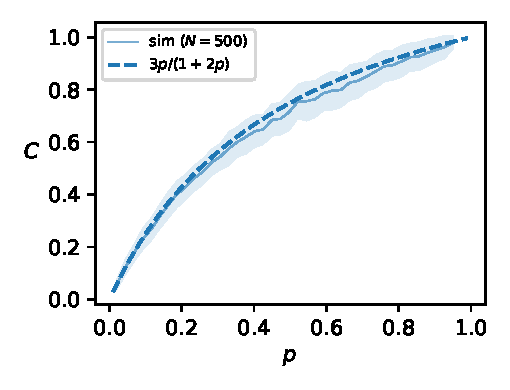
\includegraphics[width=\columnwidth]{figures/clustering.pdf}
  \caption{Global clustering coefficient $C$ as a function of $p$ for $N = 10^3$. Error bars represent one standard deviation over $10^3$ realisations. The dashed line is the analytical prediction~\eqref{eq:clustering}.}
  \label{fig:clustering}
\end{figure}

% ============================================================
\section{\label{sec:assortativity}Assortativity}
% ============================================================

The degree assortativity coefficient~\cite{newman2002} can be written as
\begin{equation}\label{eq:newman_r}
  r = \frac{4MR - S^2}{2MK_3 - S^2},
\end{equation}
where $M=M_N$, $S=\sum_i k_i^2$, $K_3=\sum_i k_i^3$, and $R=\sum_{(i,j)\in E}k_ik_j$. We already have recurrences for $M$ and $S$; a closed-form for $r$ requires tracking $K_3$ and $R$ via the same moment-closure method.

\subsection{Recurrences for higher moments}

When node $v_{\text{new}}$ is added, the target $u$ gains degree~1 (always) and each neighbour $w_i$ of $u$ gains degree~1 (with probability $p$, all or none). Accounting for degree changes of existing nodes and the new node's contribution, one obtains
\begin{align}
  K_{3,N+1} &= \!\left(1+\frac{4p}{N}\right)K_{3,N}+2+\frac{(3\!+\!6p)S_N+(6\!+\!8p)M_N}{N},\label{eq:K3_rec}\\
  R_{N+1} &= \!\left(1+\frac{4p}{N}\right)\!R_N + 1 + \frac{(1\!+\!3p)S_N+(2\!+\!6p)M_N+3pT_N}{N}.\label{eq:R_rec}
\end{align}
The derivation of~\eqref{eq:R_rec} uses the identity $\sum_u\sum_{w\sim u}\sigma_w = 2R$, where $\sigma_w = \sum_{z\sim w}k_z$, since each edge $\{w,z\}$ contributes $k_wk_z$ to both sides via the factor $k_w$.

Both recurrences share the homogeneous growth factor $(1+4p/N)$, with solution $\Phi_N = \Gamma(N+4p)/[\Gamma(1+4p)\,\Gamma(N)] \sim N^{4p}/\Gamma(1+4p)$.

\subsection{Closed-form in the sparse regime}

For $p<1/4$, all quantities $M,S,T,K_3,R$ grow linearly: $X_N\sim\alpha_X N$. Substituting this ansatz into~\eqref{eq:K3_rec}--\eqref{eq:R_rec} and using the known coefficients $\alpha_M$, $\alpha_S$, $\alpha_T$ gives
\begin{equation}
  \alpha_{K_3} = \frac{26+22p}{(1-2p)(1-3p)(1-4p)},\;\;\alpha_R = \frac{3(3+5p)}{(1-2p)(1-3p)(1-4p)}.
\end{equation}
Inserting into~\eqref{eq:newman_r}, the factors $(1-2p)$, $(1-3p)$, and $(1-4p)$ cancel between numerator and denominator, yielding
\begin{equation}\label{eq:assort}
  \boxed{r = \frac{p(9-2p)}{(1+2p)(2-p)}}, \quad p < \tfrac{1}{3}.
\end{equation}
This is derived from the exact algebraic identity $4\alpha_M\alpha_R - \alpha_S^2 = 8p(9-2p)(1-p)/[\cdots]$ and $2\alpha_M\alpha_{K_3} - \alpha_S^2 = 8(1-p)(1+2p)(2-p)/[\cdots]$, with common denominators cancelling.

The formula gives $r(0)=0$ (uncorrelated random recursive tree) and increases monotonically to $r\to 1$ as $p\to 1/3^-$. The strong assortativity near $p=1/3$ reflects the divergence of $\langle k^2\rangle$: a few high-degree hubs become mutually connected through repeated ``all'' events, dominating the degree--degree correlation. For $p\ge 1/3$, the linear-growth regime breaks down and the homogeneous terms $(\sim N^{4p})$ in $K_{3,N}$ and $R_N$ dominate; numerical simulations indicate that $r$ decreases for $p>1/3$.

\begin{figure}[h]
  \centering
  % 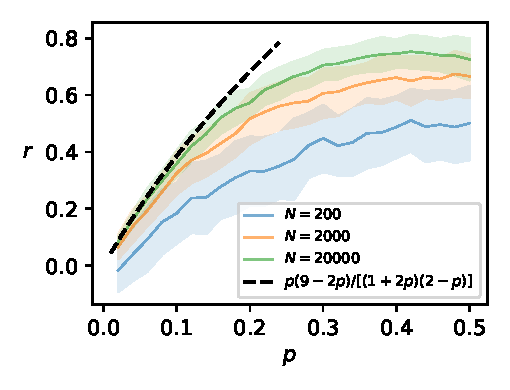
\includegraphics[width=\columnwidth]{figures/assortativity.pdf}
  \caption{Assortativity coefficient $r$ as a function of $p$ for $N = 10^3$. The dashed line is the analytical prediction~\eqref{eq:assort}.}
  \label{fig:assortativity}
\end{figure}

% ============================================================
\section{\label{sec:distance}Average Shortest-Path Distance}
% ============================================================

Unlike the previous quantities, the average shortest-path distance $\ell$ can be computed via an \emph{exact} recurrence on the total sum of pairwise distances $D_N = \sum_{i<j}d(i,j)$, without any mean-field approximation.

\subsection{Exact distance recurrence}

The key observation is that adding $v_{\text{new}}$ never shortens any existing pairwise distance (any path through $v_{\text{new}}$ can be rerouted through the target $u$ or its neighbours). When the ``all'' event occurs, $v_{\text{new}}$ acquires the \emph{same closed neighbourhood} as $u$, so for every existing node $j\neq u$, the first step on a shortest $u$--$j$ path goes through some neighbour $w$ of $u$; since $v_{\text{new}}\sim w$, we obtain $d(v_{\text{new}},j) = 1+d(w,j)=d(u,j)$ exactly. Together with $d(v_{\text{new}},u)=1$:
\begin{align}\label{eq:dist_cases}
  \text{``all'':}\;\; &\textstyle\sum_j d(v_{\text{new}},j) = 1 + \sigma_u, \nonumber\\
  \text{``none'':}\;\; &\textstyle\sum_j d(v_{\text{new}},j) = N + \sigma_u,
\end{align}
where $\sigma_u = \sum_{j\neq u}d(u,j)$ and the sums run over the $N$ existing nodes. Averaging over the uniform choice of $u$ and the binary event,
\begin{equation}\label{eq:D_rec}
  \E[D_{N+1}] = \left(1+\frac{2}{N}\right)\E[D_N] + (1-p)N+p,
\end{equation}
using $\frac{1}{N}\sum_u\sigma_u = 2D_N/N$. This recurrence is \emph{exact in expectation}, with $\E[D_1]=0$.

\subsection{Asymptotic solution}

The homogeneous solution is $\mathcal{H}_N = N(N+1)/2$. By variation of parameters, $\E[D_N] = \mathcal{H}_N\,c_N$ with partial fractions giving
\begin{equation}
  c_N = 2(2p\!-\!1)(H_N\!-\!1)+2(2\!-\!3p)\!\left(H_{N+1}-\tfrac{3}{2}\right),
\end{equation}
where $H_N = \sum_{j=1}^{N}1/j$ is the harmonic number. For large $N$, $c_N\sim 2(1-p)\ln N$, hence $\E[D_N]\sim (1-p)N(N+1)\ln N$. Dividing by $\binom{N}{2}$ pairs,
\begin{equation}\label{eq:dist_exact}
  \boxed{\ell(N) \sim 2(1-p)\ln N},
\end{equation}
valid for all $p\in[0,1)$. At $p=0$ this recovers the known Wiener-index scaling $\ell\sim 2\ln N$ of the random recursive tree; at $p=1$ the network is $K_N$ with $\ell=1$.

The distance scales \emph{logarithmically} for every $p<1$, with no phase transition. The high clustering ($C=O(1)$, Section~\ref{sec:clustering}) invalidates the locally tree-like assumption underlying the branching-process heuristic $\ell\sim\ln N/\ln\kappa$, which would incorrectly predict bounded distances for $p>1/3$. The exact recurrence~\eqref{eq:D_rec} bypasses this difficulty entirely.

\begin{figure}[h]
  \centering
  % 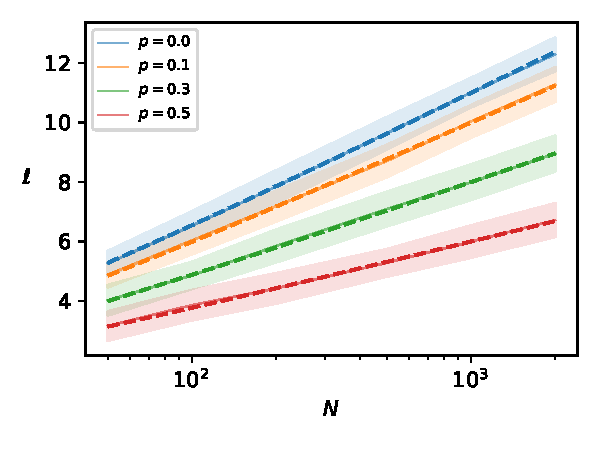
\includegraphics[width=\columnwidth]{figures/distance.pdf}
  \caption{Average shortest-path distance $\ell$ as a function of $N$ on a log-linear scale for several values of $p$. Dashed lines show the analytical prediction $2(1-p)\ln N$.}
  \label{fig:distance}
\end{figure}

% ============================================================
\section{\label{sec:conclusion}Conclusion}
% ============================================================

We have studied the all-or-none network growth model and derived exact or asymptotic analytical expressions for five structural properties, all controlled by the single parameter $p$:

(i)~The expected number of edges transitions from linear ($\sim N/(1-2p)$ for $p<1/2$) through $N\ln N$ at $p=1/2$ to superlinear ($\sim N^{2p}$) for $p>1/2$.
(ii)~The degree distribution follows a power law $P_k\sim k^{-1/p}$ with a continuously tunable exponent, matching the independent copying model at the mean-field level.
(iii)~The global clustering coefficient converges to $C=3p/(1+2p)$, a remarkably simple $N$-independent expression valid for all $p$.
(iv)~In the sparse regime ($p<1/3$), the assortativity coefficient is $r=p(9-2p)/[(1+2p)(2-p)]$, derived by moment closure, increasing from $r=0$ at $p=0$ to $r\to 1$ as $p\to 1/3^-$.
(v)~An exact topological recurrence for the sum of pairwise distances shows that the average shortest-path distance scales as $\ell\sim 2(1-p)\ln N$ for all $p<1$, with no phase transition.

The network is a \emph{small world} for every $p\in(0,1)$: logarithmic distances coexist with $O(1)$ clustering. The parameter $p$ smoothly interpolates between a random recursive tree ($p=0$) and the complete graph ($p=1$), passing through regimes that reproduce key features of real-world networks including scale-free degree distributions, tuneable assortativity, and the small-world property. Future directions include extending the assortativity formula beyond $p=1/3$, analysing the model on directed or weighted networks, and studying its spectral properties.

% ============================================================
\begin{acknowledgments}
The author thanks Professor R.\ Lambiotte for helpful discussions and the problem formulation.
\end{acknowledgments}

% ============================================================
\bibliography{references}

\end{document}
